\newpage
\section{JV editor (Steady state simulation editor)}
If you click on the JV editor icon in figure \ref{fig:ribbon_jv}, the JV editor window will open shown below in figure \ref{fig:jvcurveeditor}.

\begin{figure}[H]
\centering
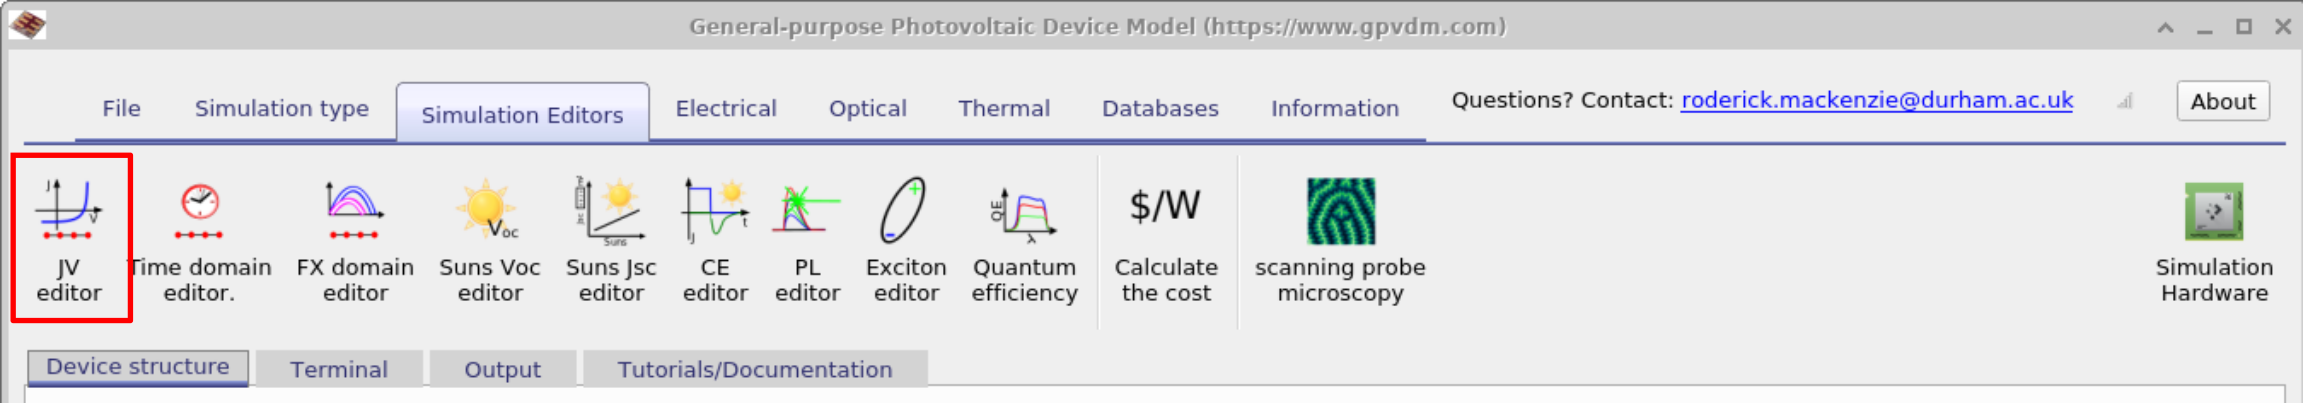
\includegraphics[width=0.8\textwidth]{./images/sim_editors/ribbon_jv.png}
\caption{Opening the JV editor from the simulation editor ribbon.}
\label{fig:ribbon_jv}
\end{figure}

\subsection{Inputs}

This window can be used to configure steady state simulations. It does not matter if you are running a current-voltage sweep on a solar cell or an OFET.  This plugin will steadily ramp the voltage from a start voltage to a stop voltage.  The voltage will be applied to the contact which has been set to \emph{Change} in the contact editor (see section \ref{sec:contacteditor}). You can set the start voltage, stop voltage and step size.  Use \emph{JV voltage step multiplayer} to make the voltage step grow each step.  The default is 1.0, i.e. no growth. It can be helpful to set the step multiplyer to a value larger than 1.0 if you want to speed up the simulation but it should not be increased past about 1.05 or the simulation may strugle to converge.

\begin{figure}[H]
\centering
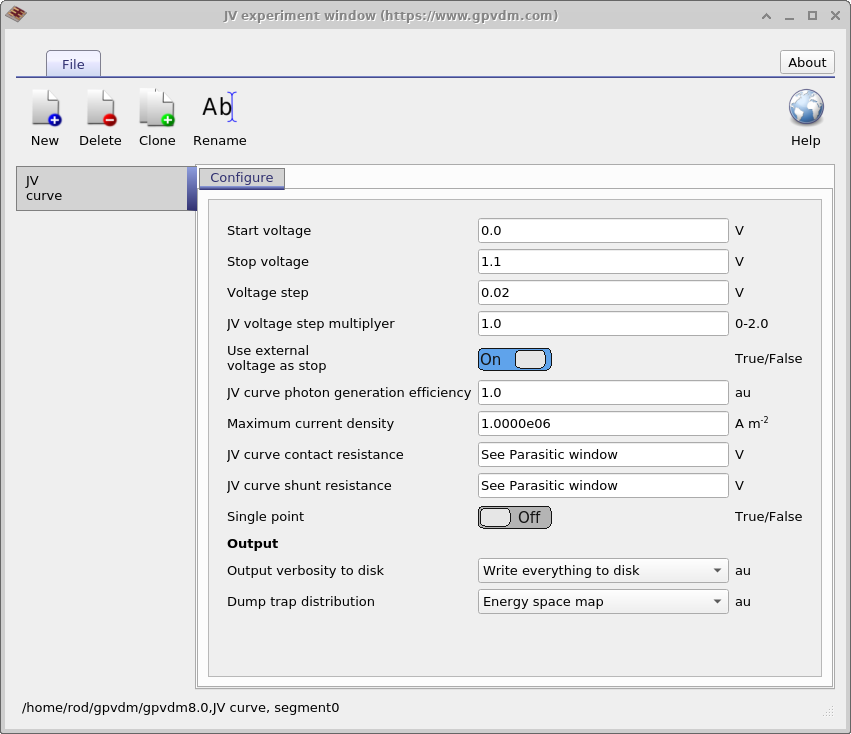
\includegraphics[width=0.7\textwidth,height=0.6\textwidth]{./images/sim_editors/jv_editor.png}
\caption{The JV editor editor window, use this to configure steady state simulations.}
\label{fig:jvcurveeditor}
\end{figure}

\subsection{Outputs}
The files produced by the JV simulation mode are given in table \ref{tab:jv_output}. As well as these files, by default OghmaNano will also write all internal simulation parameters to disk in the snapshots directory. This includes band structure, potential, carrier distributions, generation rates etc.. this equates to about 50 files per voltage step. You can read more about this in the simulation snapshots section, see \ref{sec:snapshots}. This can considerably slow down the simulation, the user can therefore decide how much is written to disk by using the \emph{Output verbosity to disk option} this can be set to; \emph{Key results}, which will result in only key files being written to disk;\emph{Nothing}, which will result in no results being written to disk; \emph{Write everything to disk} which will result in a all possible information being written to disk and \emph{Write everything to disk every nth step}, which will only out comprehensive internal simulation write data every nth step.

\begin{table}[H]
\begin{center}
\begin{tabular}{ |c|c|c| } 
 \hline
	File name 			& 	Description  \\ 
 \hline
	$jv.dat$ 			&	Current voltage curve \\ 
	$charge.dat$ 		&	voltage charge density\\ 
	$k.csv$ 			&	Recombination constant k\\ 
	$sim\_info.dat$ 	&	Calculated $V_{oc}$, $J_{sc}$ etc.. see \ref{sec:siminfo}   \\

 \hline
\end{tabular}
\caption{Files produced by the JV simulation}
\label{tab:jv_output}
\end{center}
\end{table}

\subsection{sim\_info.dat}
\label{sec:siminfo}
This is a json file containing all key simulation metrics such as $J_{sc}$, $V_{oc}$, and example sim\_info.dat file is given below:


\subsection{Steady state electrical simulation}
\label{sec:siminfo}
In steady state electrical simulations such as performing a JV scan the sim\_info.dat outputs the following parameters.

\begin{landscape}
\begin{center}
\begin{tabular}{ |c|c|c|c| c| c|} 
\hline
Symbol & JSON token & Meaning & Units & Equ. & Ref \\
\hline
FF 				& ff 			& Fill factor										&au			&&\\
PCE 			& pce 			& PCE& percent										&			&\\
$P_{max}$ 		& $P\_{max}$ 	& Power at Pmax										&			&&\\
$V_{oc}$ 		& $V\_{oc}$ 		& $V_{oc}$ 										&			&&\\
$voc_{R}$ 		& $voc\_{R}$ 	& Recombination rate at $P_{max}$ 					&			& &\\
$jv_{voc}$  	& $jv\_{voc}$  	& 													&			&&\\
$jv_{pmax}$ 	& $jv\_{pmax}$ 	& 													&			&&\\
$voc_{nt}$ 		& $voc\_{nt}$ 	& Trapped electron carrier densiyt at $V_oc$		&			&&\\
$voc_{pt}$ 		& $voc\_{pt}$ 	& Trapped hole carrier density at $V_oc$			&			&&\\
$voc_{nf}$ 		& $voc\_{nf}$ 	& Free electron carrier densiyt at $V_oc$			&			&&\\
$voc_{pf}$ 		& $voc\_{pf}$ 	& Free hole carrier density at $V_oc$				&			&&\\
$J_{sc}$   		& $J\_{sc}$   	& $J_{sc}$											&$Am^{-2}$ 	& &\\
$jv_{jsc}$ 		& $jv\_{jsc}$ 	& Average charge density at $J_{sc}$				&$m^{-3}$ 	& &\\
$jv_{vbi}$ 		& $jv\_{vbi}$ 	& Built in voltage									& V			&&\\
$jv_{gen}$ 		& $jv\_{gen}$ 	& Average generation rate							&			&&\\
$voc_{np}$ 		& $voc\_{np}$ 	& 													&			&&\\
$j_{pmax}$ 		& $j\_{pmax}$ 	& Current at $P_{max}$								&$Am^{-2}$ 	& &\\
$v_{pmax}$ 		& $v\_{pmax}$ 	& Voltage at $P_{max}$    							&V			&  &\\
\hline
\end{tabular}
\end{center}

%Tau
\begin{center}
\begin{tabular}{ |c|c|c|c| c| c|} 
\hline
Symbol & JSON token & Meaning & Units & Equ. & Ref \\
\hline

%Mobility
$\mu_{jsc}$ 				& $mu\_{jsc}$ 				& Avg. mobility at $J_{sc}$				&$m^{2} V^{-1} s^{-1}$ 	&&\\
$\mu^{geom}_{jsc}$ 			& $mu\_geom\_jsc$ 			& Geom. avg. mobility @ $J_{sc}$		&$m^{2} V^{-1} s^{-1}$ 	&&\\
$\mu^{geom\_micro}_{jsc}$ 	& $mu\_geom\_micro\_jsc$ 	& Geom. avg. mobility @ $J_{sc}$		&$m^{2} V^{-1} s^{-1}$ 	&&\\


$\mu_{voc}$ 				& $mu\_{voc}$ 				& Average mobility @ $V_{oc}$			& $m^{2} V^{-1} s^{-1}$ &&\\
$\mu^{geom}_{voc}$ 			& $mu\_geom\_voc$ 			& Geom. avg. mobility @ $V_{oc}$		& $m^{2} V^{-1} s^{-1}$ &$\sqrt{\langle\mu_e\rangle \langle\mu_h\rangle}$&\\
$\mu^{geom\_avg}_{voc}$ 	& $mu\_geom\_micro\_voc$ 	& Geom. avg. mobility @ $V_{oc}$		& $m^{2} V^{-1} s^{-1}$ &$\langle\sqrt{mu_e \mu_h}\rangle$&\\

$\mu^e_{pmax}$ 				& $mu\_e\_{pmax}$ 			& Avg. electron mobility @ $P_{max}$	&$m^{2} V^{-1} s^{-1}$ 	&&\\
$\mu^h_{pmax}$ 				& $mu\_h\_{pmax}$ 			& Avg. hole mobility @ $P_{max}$ 		&$m^{2} V^{-1} s^{-1}$ 	&&\\
$\mu^{geom}_{pmax}$ 		& $mu\_geom\_pmax$ 			& Geom. avg. mobility @ $P_{max}$ 		&$m^{2} V^{-1} s^{-1}$ 	&$\sqrt{\langle\mu_e\rangle \langle\mu_h\rangle}$&\\
$\mu^{geom\_micro}_{pmax}$ 	& $mu\_geom\_micro\_pmax$ 	& Geom. avg. mobility @ $P_{max}$ 		&$m^{2} V^{-1} s^{-1}$ 	&$\langle\sqrt{mu_e \mu_h}\rangle$&\\
$\mu^{pmax}$ 				& $mu\_{pmax}$ 				& Avg. mobility @ $P_{max}$				&$m^{2} V^{-1} s^{-1}$ 	&&\\
\hline
\end{tabular}

\end{center}

%Tau
\begin{center}
\begin{tabular}{ |c|c|c|c| c| c|} 
\hline
Symbol & JSON token & Meaning & Units & Equ. & Ref \\
\hline


$\tau_{voc}$ 	& $tau\_{voc}$ 	&	Recom. time at $V_{oc}$	 			& s 		&	$R=(n-n0)/\tau$  & \cite{doi:10.1021/jp073056p}\\
$\tau_{pmax}$ 	& $tau\_{pmax}$ &	Recom. time at $P_{max}$				&s 			&	$R=(n-n0)/\tau$  & \cite{doi:10.1021/jp073056p}\\
$\tau_{voc}^{all}$ 	& $tau\_all\_{voc}$ 	&	Recomb. time at $V_{oc}$	& s 		&	$R=(n)/\tau$  & \cite{doi:10.1021/jp073056p}\\
$\tau_{pmax}^{all}$ 	& $tau\_all\_{pmax}$ &	Recomb. time at $P_{max}$	&s 			&	$R=(n)/\tau$  & \cite{doi:10.1021/jp073056p}\\
\hline

%Ivan's stuff
$theta_{srh}$ 	&$theta\_{srh}$ & $\theta_{SRH}$ Collection coefficient at $P_{max}$ y & au &&p.100 5.2a\cite{Summon-FETCH-bonn_catalog_45326403},\cite{PhysRevApplied.6.024001}\\
$theta_{srh}$ 	&$theta\_{srh}$ & $\theta_{SRH}$ Collection coefficient at $P_{max}$ & au &&p.100 5.2a\cite{Summon-FETCH-bonn_catalog_45326403},\cite{PhysRevApplied.6.024001}\\


\hline
\end{tabular}

\end{center}

\end{landscape}


